\chapter*{Appendix}\label{ch:appendix}
\addcontentsline{toc}{chapter}{Appendix}
\renewcommand{\thesection}{A.\arabic{section}}


\section{Mathematical derivations}\label{sec:derivations}


\begin{proposition*}[Proposition \ref{prop:analytical}]
    When the transition rates are constant, we can compute the analytical solution of Equation \ref{eq:proportions}, depending on the values of $p$ and $q$, is as follows.
    \begin{itemize}
        \item If $p\neq q$, the solution is
            \begin{align*}
                \begin{dcases}
                    \phi_A = ae^{-pt}\\
                    \phi_B = \frac{ap}{q-p}\left(e^{-pt}-e^{-qt}\right)+(1-a)e^{-qt}\\
                    \phi_C = \frac{a}{q-p}\left(-qe^{-pt}+pe^{-qt}\right) - (1-a)e^{-qt} + 1
                \end{dcases}
            \end{align*}

        \item If $p=q$, the solution is
            \begin{align*}
                \begin{dcases}
                    \phi_A = ae^{-pt}\\
                    \phi_B = e^{-pt}(apt + 1 - a)\\
                    \phi_C = e^{-pt}(-1-apt) + 1
                \end{dcases}
            \end{align*}
    \end{itemize}
\end{proposition*}

\begin{proof}
    \hfill
    \begin{enumerate}
        \item The expression for $\phi_A$ is solved as follows,
        \begin{align*}
            \int\frac{\diff\phi_A}{\phi_A}&=\int-pdt,\\
            \ln(\phi_A)&=-pt+C,\\
            \phi_A&=Ke^{-pt}.
        \end{align*}
        Imposing $\phi_A(0)=a$, we get $K=a$.

        \item To solve $\phi_B$, we first multiply the differential equation by the integrating factor $e^{qt}$,
        \begin{align*}
            e^{qt}\dot\phi_B+e^{qt}q\phi_B&=pe^{qt}\phi_A,\\
            \frac{d}{dt}(e^{qt}\phi_B)&=pe^{qt}\phi_A,\\
            e^{qt}\phi_B&=\int pe^{qt}\phi_A dt,\\
            \phi_B&=pe^{-qt}\int ae^{(q-p)t}dt.
        \end{align*}

        \begin{itemize}

            \item If $p\neq q$,
            \begin{align*}
                \phi_B &\underset{\phantom{\phi_B(0) = 1-a}}{=} ape^{-qt}\int e^{(q-p)t}dt\\
                &\underset{{\phantom{\phi_B(0) = 1-a}}}{=} ape^{-qt}\left(\frac{1}{q-p}e^{(q-p)t}+C\right) \\
                &\underset{\phi_B(0) = 1-a}{=} ape^{-qt}\left(\frac{1}{q-p}e^{(q-p)t}
                +\frac{1-a}{ap}-\frac{1}{q-p}\right)\\
                &\underset{\phantom{\phi_B(0) = 1-a}}{=} \frac{ap}{q-p}\left(e^{-pt}-e^{-qt}\right)+(1-a)e^{-qt}.
            \end{align*}

            \item If $p=q$,
            \begin{align*}
                \phi_B &\underset{\phantom{\phi_B(0) = 1-a}}{=} ape^{-pt}\int e^{(p-p)t}dt = ape^{-pt}(t + C)\\ 
                &\underset{\phi_B(0) = 1-a}{=} e^{-pt}(apt + 1 - a).
            \end{align*}

        \end{itemize}

        \item Solving for $\phi_C$ reads
        \begin{align*}
            \phi_C = q\int\phi_B dt.
        \end{align*}

        \begin{itemize}
            
            \item If $p\neq q$, then
            \begin{align*}
                \phi_C &\underset{\phantom{\phi_B(0) = 0}}{=}
                \frac{qap}{q-p}\int{(e^{-pt}-e^{-qt})dt}+q(1-a)\int{e^{-qt}dt}\\
                &\underset{\phantom{\phi_B(0) = 0}}{=}
                \frac{qap}{q-p}\left(-\frac{e^{-pt}}{p}+\frac{e^{-qt}}{q}\right) - (1-a)e^{-qt} + C\\
                &\underset{\phi_C(0) = 0}{=}
                \frac{a}{q-p}\left(-qe^{-pt}+pe^{-qt}\right) - (1-a)e^{-qt} + 1.
            \end{align*}

            \item If $p=q$, then
            \begin{align*}
                \phi_C &\underset{\phantom{\phi_B(0) = 0}}{=}p\int{e^{-pt}(apt + 1 - a) dt}\\
                &\underset{\phantom{\phi_B(0) = 0}}{=}
                pa\int{e^{-pt}pt dt} + p(1 - a)\int{e^{-pt}dt}\\
                &\underset{\phantom{\phi_B(0) = 0}}{=}
                pa\left( -e^{-pt}t - \frac{e^{-pt}}{p}\right) - (1-a)e^{-pt} + C\\
                &\underset{\phi_C(0)=0}{=} 
                e^{-pt}\left(-1-apt\right) + 1.
            \end{align*}
        \end{itemize}
    \end{enumerate}
\end{proof}


\begin{proposition}[Proposition \ref{prop:nondim}]
    The dimensionless equations of motion are
    \begin{align}\tag{\ref{eq:motion}}
        \begin{aligned}
            \tilde \lambda \tilde v_i &=\sum_{j=1}^{N}\tilde F_{ij} + P_k \tilde F_{p_i}\\
            \frac{\diff \tilde x_i}{\diff\tilde t} &=\tilde v_i,
        \end{aligned}
    \end{align}
    with initial conditions
    \begin{equation}\tag{\ref{eq:motion}}
        \tilde v_i(0) = \tilde v_{0_i}, \qquad \tilde x_i(0) = \tilde x_{0_i}.
    \end{equation}
\end{proposition}

\begin{proof}
    \hfill
    \begin{enumerate}
        \item Substituting the previous expressions into the first equation of \ref{eq:motion_dim} leads to
        \begin{align*}
            \left(\tilde{\lambda}\frac{F_0T_0}{R_0}\right) \left(\tilde{v}_k\frac{R_0}{T_o}\right) = \sum_{j=1}^{N} F_0\tilde F_{ij}+ F_0 P_i\tilde F_p,
        \end{align*}
        and constants cancel out leading to the described equation.
        \item Substituting the previous expressions into the second equation of \ref{eq:motion_dim} leads to
        \begin{align*}
            \frac{\diff \left(\tilde{x}_i R_0\right)}{\diff(\tilde t T_0)} = \tilde v_i \frac{R_0}{T_0},
        \end{align*}
        and constants cancel out leading to the described equation.
    \end{enumerate}
\end{proof}



\section{Code}\label{sec:code}

\subsection{Technical specifications}\label{sec:specs}

Computations have been carried out using the system configuration described in Table \ref{tab:specs}.

\begin{table}[ht]
    \centering
    \begin{tabular}{|l|l|}
        \hline
        Device & \textit{Lenovo Ideapad 5-15ITL05 (82FG)} \\ \hline
        OS & \textit{Linux Mint 22 Cinnamon (6.2.9)} \\ \hline
        Julia & \textit{Julia 1.9.4+0.x64.linux.gnu} \\ \hline
        CBM.jl & \textit{CellBasedModels v0.1.0} \\ \hline
    \end{tabular}
    \caption{Technical specifications.}
    \label{tab:specs}
\end{table}
    

\subsection{Programs}\label{sec:programs}

All the code has been written in Julia using Jupyter Notebooks unless stated otherwise.


\begin{program}[\code{preamble/packages}]\label {pg:packages}
    Loads the packages needed for the project.
\end{program}

\begin{program}[\code{preamble/model}]\label{pg:model}
    Loads the global friction model (see Equation \ref{eq:motion}).
\end{program}

\begin{program}[\code{preamble/functions}]\label{pg:functions}
    Loads most of the functions used by the programs.
\end{program}

\begin{program}[\code{3.01}]\label{pg:niproblem-avg}
    Visualization of the issue regarding the increase of neighbours. Averaged over several realizations.
\end{program}
    
\begin{program}[\code{3.02}]\label{pg:niproblem}
    Analysis of the issue regarding the increase of neighbours.
\end{program}

\begin{program}[\code{3.03}]\label{pg:solution-varfriction}
    Parameter sweep for $\alpha_\text{adh}$ using the variable friction model.
\end{program}

\begin{program}[\code{3.04}]\label{pg:solution-ctfriction}
    Parameter sweep for $\alpha_\text{adh}$ using the constant friction model
\end{program}

\begin{program}[\code{3.05}]\label{pg:proposal}
    Proposed model with constant fiction.
\end{program}

\begin{program}[\code{3.06}]\label{pg:unstable-vsum}
    Instability of the model using Equation \ref{eq:worst}.
\end{program}

\begin{program}[\code{3.07}]\label{pg:vsum-zero}
    Computation of the sum of velocities of the neighbours using the model introduced in Program \ref{pg:solution-varfriction}.
\end{program}

\begin{program}[\code{4.00}]\label{pg:example-code}
    Example displaying the main features and functions of the code.
\end{program}

\begin{program}[\code{4.01}]\label{pg:formed-correctly}
    Loop that simulates communities using different parameters in order to perform parameter sweep and ensure stability.
\end{program}

\begin{program}[\code{4.02}]\label{pg:growdiff}
    Simulation assuming that proliferation continues during differentiation.
\end{program}

\begin{program}[\code{4.03}]\label{pg:measure-growth}
    Measurement of the growth of cells.
\end{program}

\begin{program}[\code{4.04}]\label{pg:measure-protrusions}
    Measurement of the effect of protrusions.
\end{program}

\begin{program}[\code{4.05}]\label{pg:proportions}
    Average of the proportions of cell types for several realizations and comparison of the output to known solutions. It includes computations for several configurations.
\end{program}

\begin{program}[\code{4.06}]\label{pg:growdiff-proportions}
    Replica of the computations performed in Program \ref{pg:proportions} using the set-up described in Program \ref{pg:growdiff}.
\end{program}

\begin{program}[\code{4.07} and \code{4.08}]\label{pg:phib}
    Computation of the proportion of cells in state B in terms of its initial proportion for a given set of timestamps, and comparison with known solutions. For a single realization in \code{4.07}, and averaged in \code{4.08}.
\end{program}

\begin{program}[\code{4.09}]\label{pg:adh}
    Simulation assuming that force between two cells can change depending on their states. Plots the cells in each state to visualize the effect.
\end{program}

\begin{program}[\code{4.10}]\label{pg:adh-avgs}
    Replica of the computations performed in Programs \ref{pg:proportions} and \ref{pg:phib} using the set-up described in Program \ref{pg:adh}.
\end{program}

\begin{program}[\code{4.11}]\label{pg:adh-growing}
    Replica of the computations performed in Programs \ref{pg:proportions} using the set-up described in Program \ref{pg:adh} along with proliferation during the differentiation process.
\end{program}

\begin{program}[\code{images2gif.py}]\label{pg:script}
    Python script that finds plots in the folder and converts them into a GIF.
\end{program}


\subsection{Packages}

The main package, \code{CellBasedModels.jl}, already includes some features such as numerical integrators and probability distributions. However, some tasks require extra packages.
\begin{itemize}
    \item All plots are created using \code{GLMakie} \parencite{Makie_2021}, and formatted with \code{MathTeXEngine}. The colours used are from the colour-blind friendly palette presented in \cite{Wong_2011}.
    \item Sampling and random seeds are provided by \code{Distributions} and \code{Random}, respectively.
    \item File formatting is handled by the packages \code{Printf} and \code{Dates}, and data extraction by \code{Glob}.
    \item Preamble files are included in the program using \code{NBInclude}.
    \item The Python script (see Program \ref{pg:script}) requires the \code{imageio} package.
\end{itemize}


\section{Additional figures}\label{sec:supp}

Figure \ref{fig:phix-solutions} corresponds to the proportion of cells in states $A$ and $C$ in terms of $\phi_B(0)=b$. The analogous plot for $B$ is studied in section \ref{sec:phi-b}.

\begin{figure}[ht]
    \centering
    \begin{subfigure}{0.4\textwidth}
        \centering
        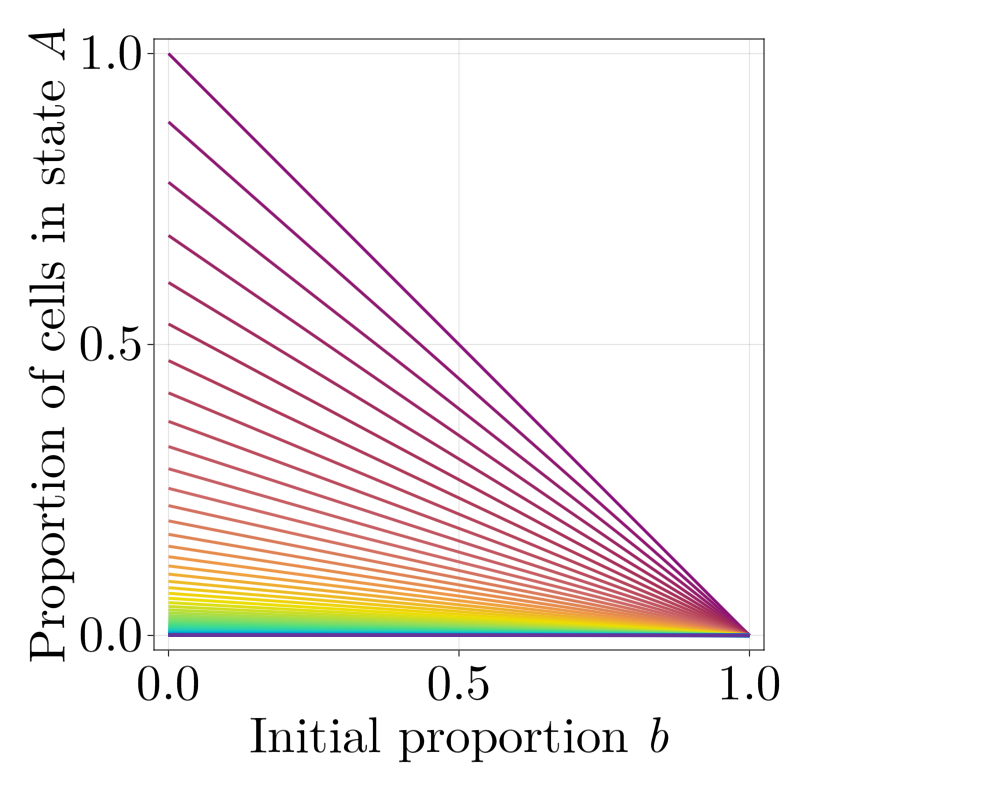
\includegraphics[width=\textwidth]{figures/407/407-phia-vs-b-solution-constant-all.png}
        % \caption{Constant rates,\\time $t=0,1,...,60$ (h).}
    \end{subfigure}
    \hspace{5em}
    \begin{subfigure}{0.4\textwidth}
        \centering
        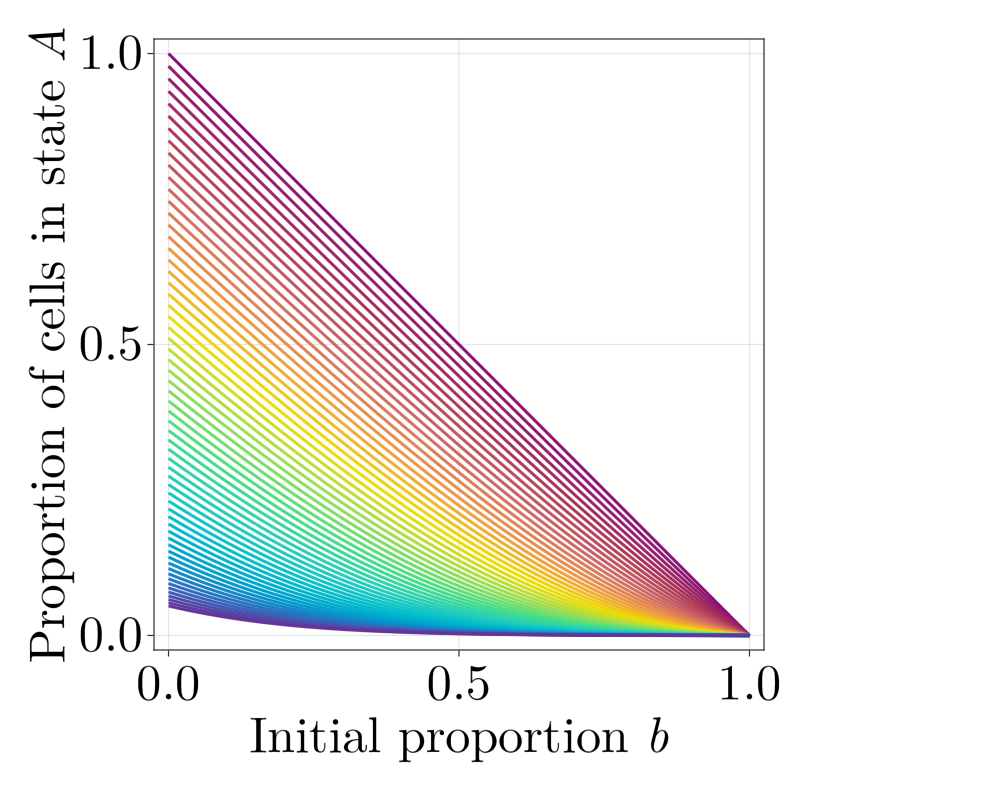
\includegraphics[width=\textwidth]{figures/407/407-phia-vs-b-solution-meanfield-all.png}
        % \caption{Mean field feedback,\\time $t=0,1,...,60$ (h).}
    \end{subfigure}
    \\
    \begin{subfigure}{0.4\textwidth}
        \centering
        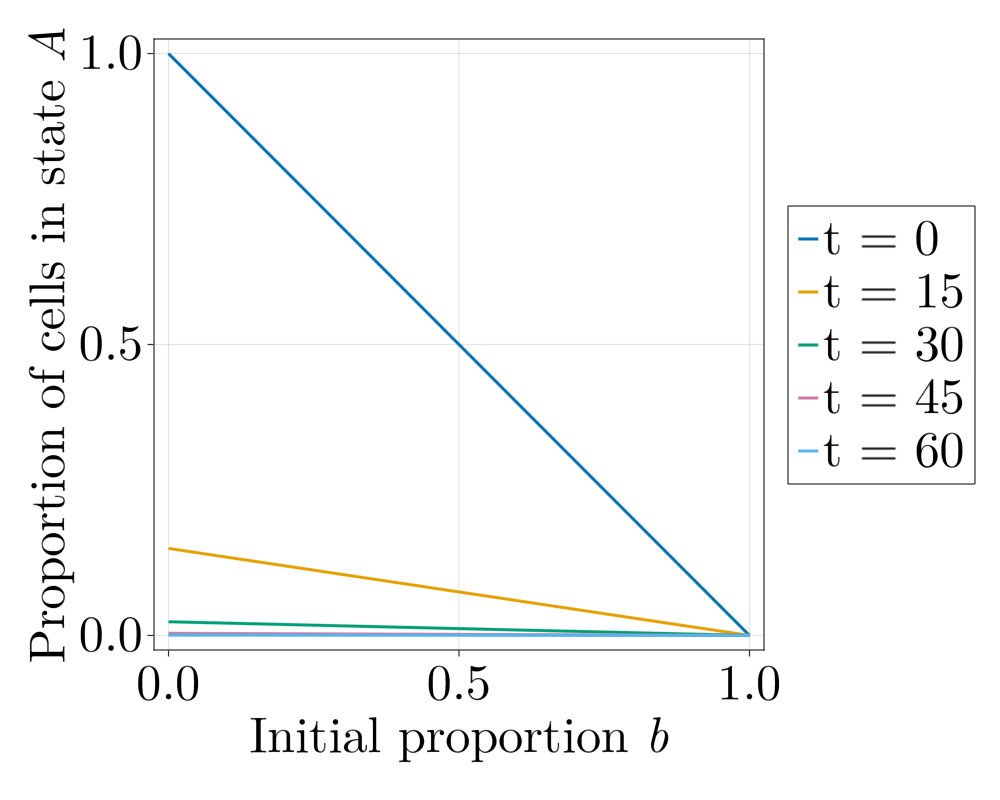
\includegraphics[width=\textwidth]{figures/407/407-phia-vs-b-solution-constant.png}
        % \caption{Constant rates.}
    \end{subfigure}
    \hspace{5em}
    \begin{subfigure}{0.4\textwidth}
        \centering
        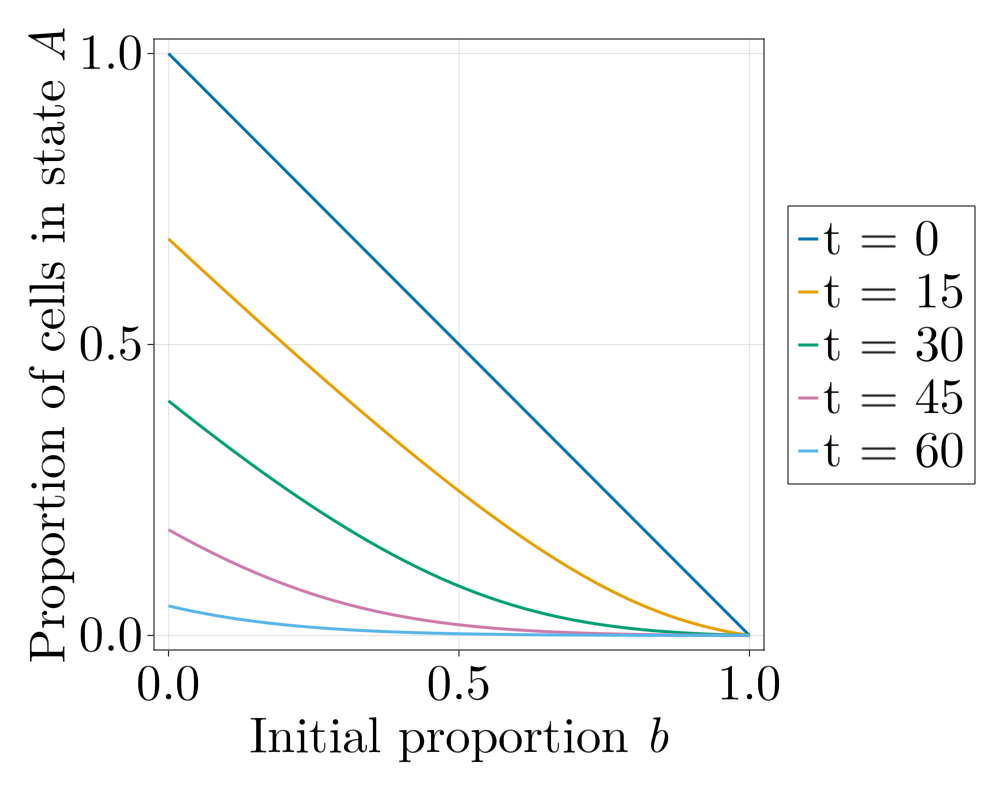
\includegraphics[width=\textwidth]{figures/407/407-phia-vs-b-solution-meanfield.png}
        % \caption{Mean field feedback.}
    \end{subfigure}
    \\
    \begin{subfigure}{0.4\textwidth}
        \centering
        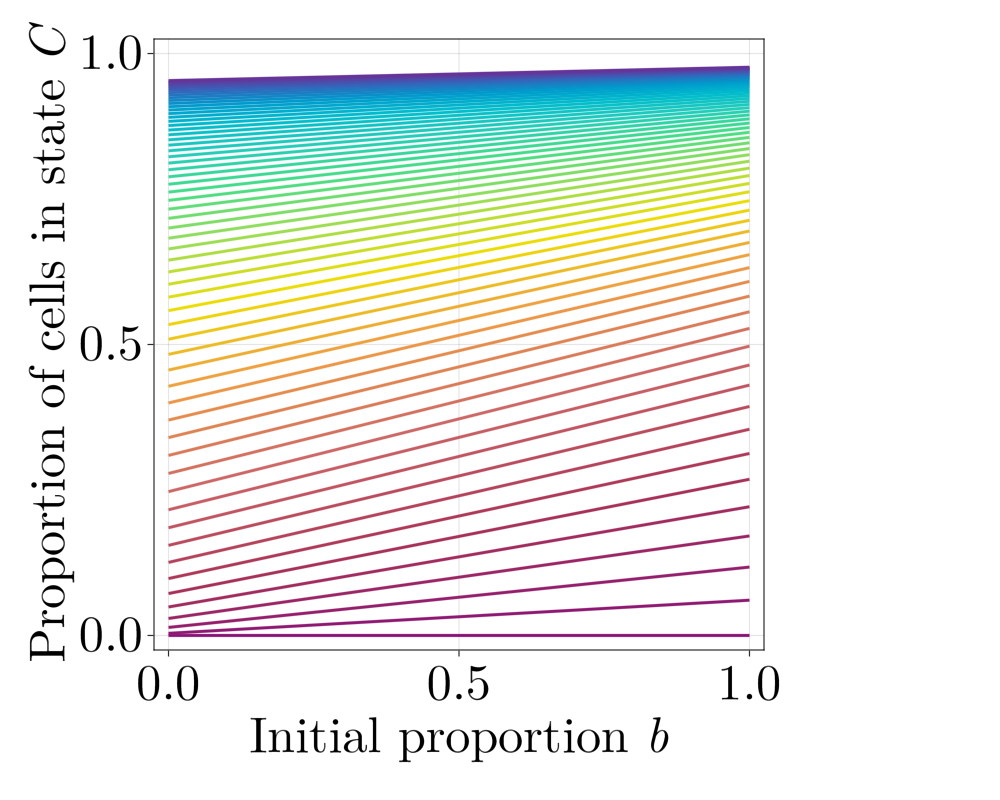
\includegraphics[width=\textwidth]{figures/407/407-phic-vs-b-solution-constant-all.png}
        % \caption{Constant rates,\\time $t=0,1,...,60$ (h).}
    \end{subfigure}
    \hspace{5em}
    \begin{subfigure}{0.4\textwidth}
        \centering
        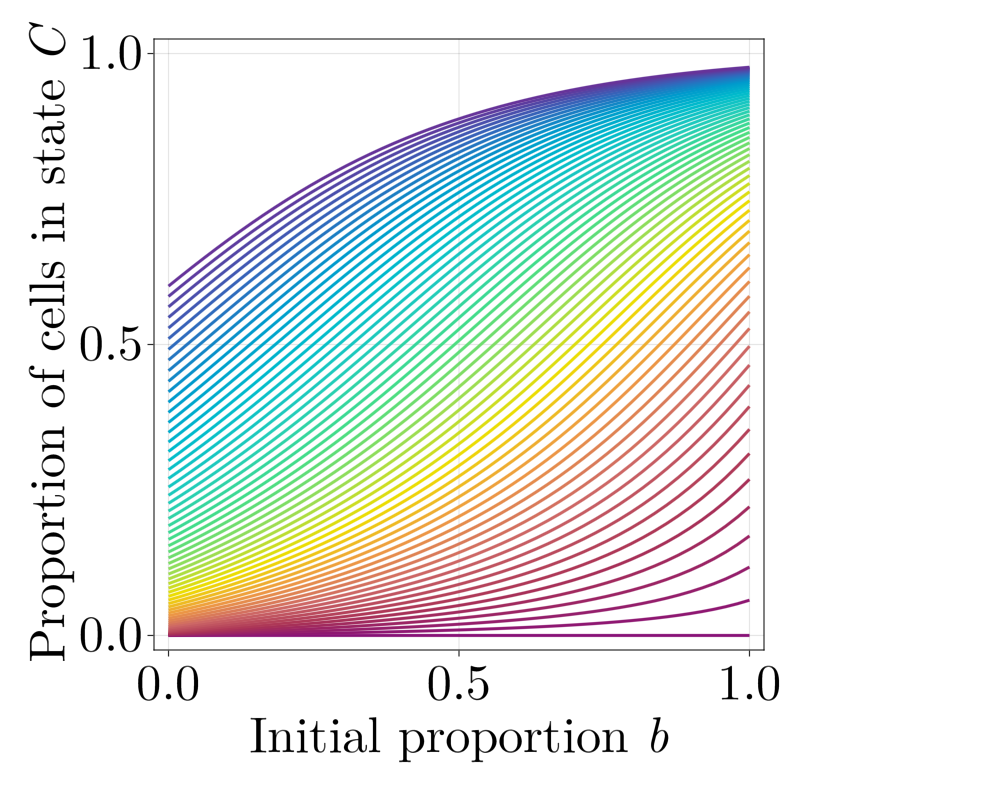
\includegraphics[width=\textwidth]{figures/407/407-phic-vs-b-solution-meanfield-all.png}
        % \caption{Mean field feedback,\\time $t=0,1,...,60$ (h).}
    \end{subfigure}
    \\
    \begin{subfigure}{0.4\textwidth}
        \centering
        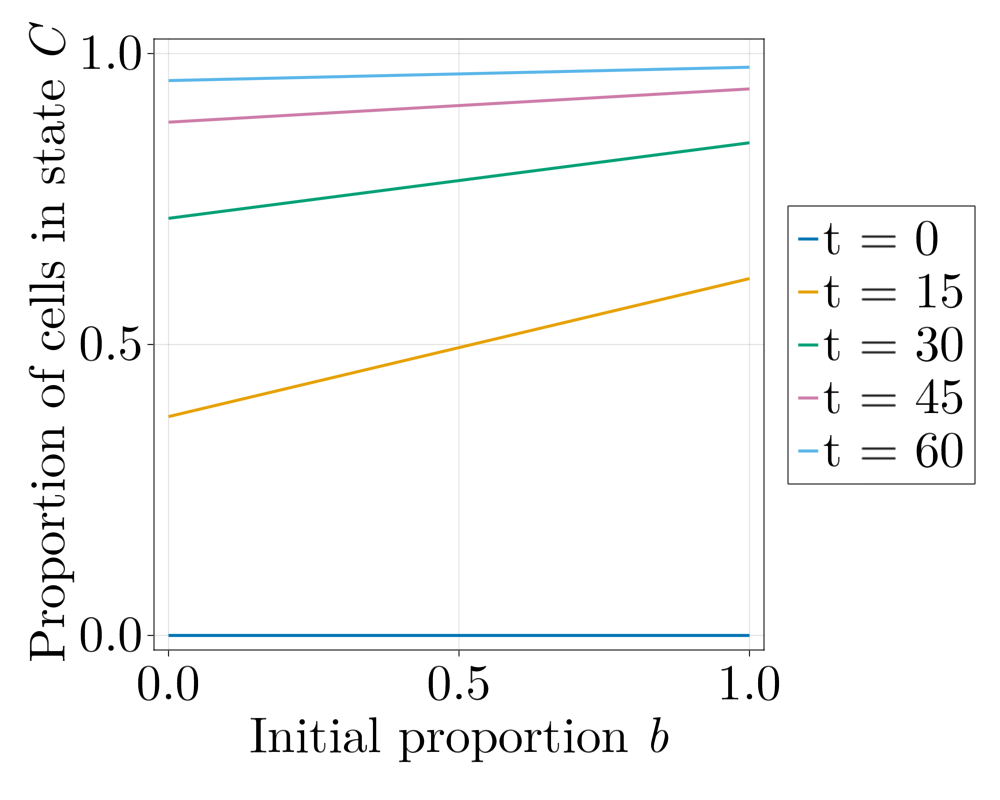
\includegraphics[width=\textwidth]{figures/407/407-phic-vs-b-solution-constant.png}
        % \caption{Constant rates.}
    \end{subfigure}
    \hspace{5em}
    \begin{subfigure}{0.4\textwidth}
        \centering
        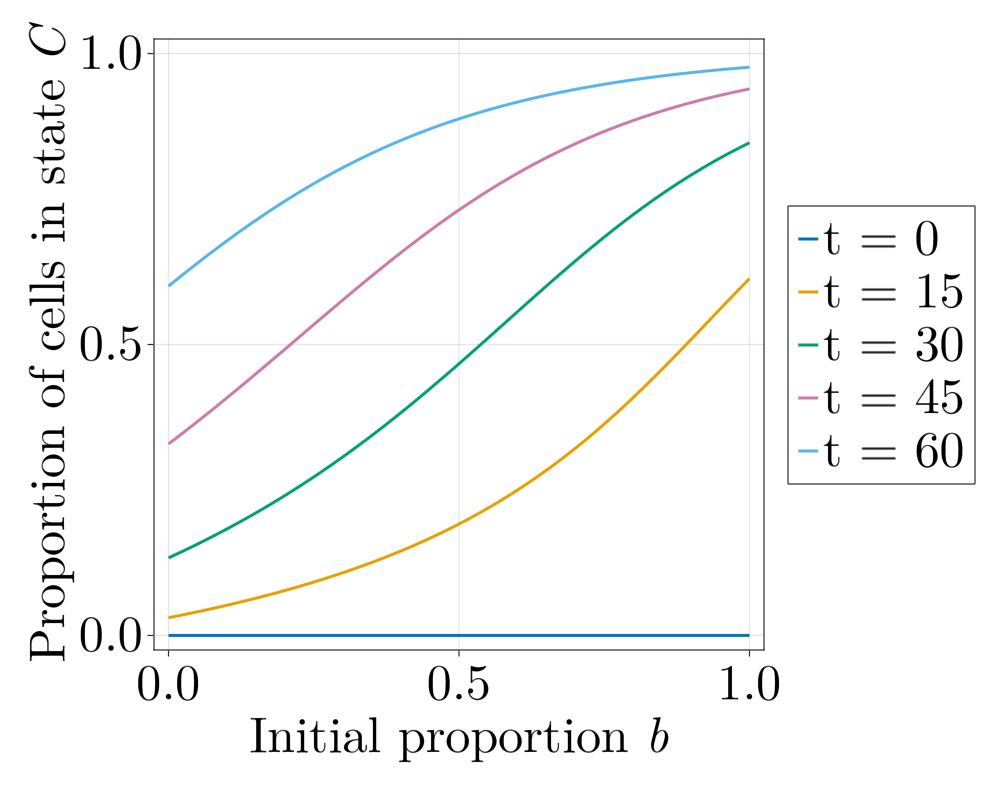
\includegraphics[width=\textwidth]{figures/407/407-phic-vs-b-solution-meanfield.png}
        % \caption{Mean field feedback.}
    \end{subfigure}
    \caption{$\phi_X(t_n)$ against $b$ using the known solutions, $X=A,B$ for constant rates (left) and mean field feedback (right). Plots for each second $s\in[0,60]$ when unspecified.}
    \label{fig:phix-solutions}
\end{figure}